\chapter{Rezultaty pomiarów}
Testy całego systemu pomiarowego zostały przeprowadzone w dwóch różnych środowiskach. W pierwszym przypadku mierzone były warunki atmosferyczne panujące na zewnątrz budynku mieszkalnego. Drugi test został przeprowadzony w warunkach mieszkalnych.
\section*{Środowisko naturalne}
Cały układ pomiarowy został testowo wykorzystany do badania warunków  meteorologicznych panujących na wolnym powietrzu. Aplikacja zbierająca dane została uruchomiona na kilka godzin (od około 15:00 do 21:00).

Poniższe wykresy prezentują warunki wtedy panujące. Jak widać na załączonych rysunkach, temperatura stale maleje wraz z upływem czasu. Świadczy to o poprawnym pomiarze, gdyż 
\begin{figure}[h!]
\centering
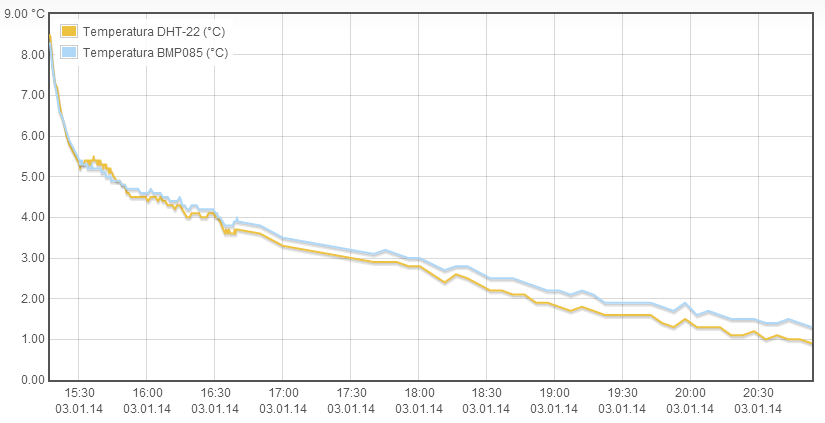
\includegraphics[scale=0.65]{zewnatrz_temp}
\caption{Pomiar temperatury na zewnątrz budynku}
\label{fig:zewnatrz_temp}
\end{figure}

\begin{figure}[h!]
\centering
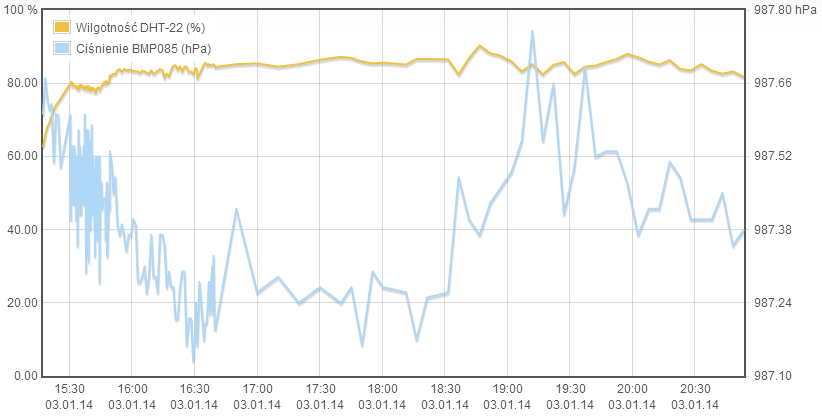
\includegraphics[scale=0.65]{zewnatrz_reszta}
\caption{Pomiar wilgotności oraz ciśnienia na zewnątrz budynku}
\label{fig:zewnatrz_temp}
\end{figure}

\section*{Warunki pokojowe}
\begin{figure}[h!]
\centering
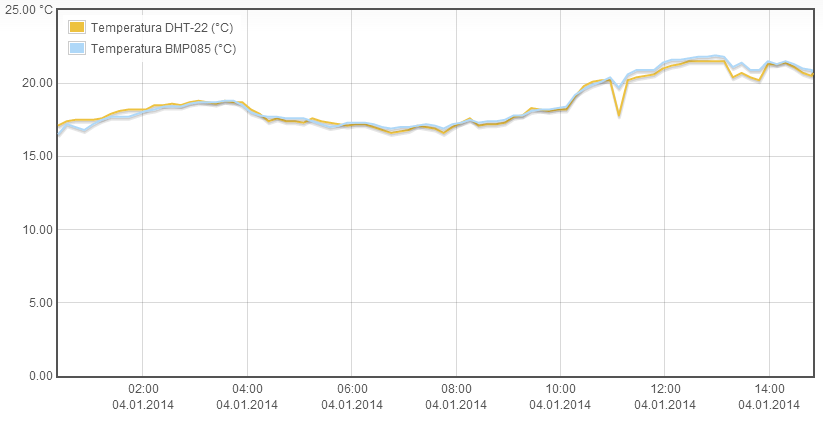
\includegraphics[scale=0.65]{wewnatrz_temp}
\caption{Pomiar temperatury wewnątrz pomieszczenia}
\label{fig:zewnatrz_temp}
\end{figure}

\begin{figure}[h!]
\centering
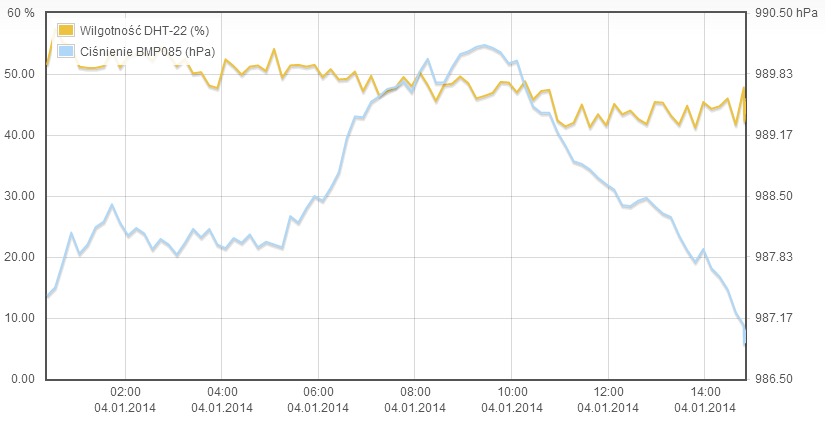
\includegraphics[scale=0.65]{wewnatrz_reszta}
\caption{Pomiar wilgotności oraz ciśnienia wewnątrz pomieszczenia}
\label{fig:zewnatrz_temp}
\end{figure}